%*******************************************************************************
%****************************** Second Chapter *********************************
%*******************************************************************************

\chapter{Evaluation on toy models}
So far we have considered two variational approaches to the general Boltzmann distribution where pair-wise connections might be defined between all nodes in the graph. However, we are interested in the adaptation of the extended mean field approximation to the restricted Boltzmann machine.

\section{Adaptation of EMF to RBM}
Adaptation of the extended mean field approximation derived in the first chapter to the case of the RBM is rather straightforward. Let's divide set of spins into visible  and hidden variables along with corresponding biases ($a$ and $b$ for visible and hidden units respectively). We will denote by $\mathbf{m}^\mathbf{v} = \{m_i \}_{i=1}^N$ and $\mathbf{m}^\mathbf{h} = \{m_i \}_{j=1}^M$ corresponding sets of magnetizations where $N$ and $M$ are the sizes of the visible and hidden layers accordingly. The energy in the BM models is set to $1$ thus we set $\beta$ to $1$ as well. This leads to the following free energy expansion (up to the third term) in the new setting:
\begin{align}
\begin{split}
F^{EMF}(\mathbf{m^v},\mathbf{m^h}) ~\simeq & ~H(\mathbf{m^v}, \mathbf{m^h}) \\
&  - \sum_i a_i m_i^v - \sum_j b_j m_j^h \\
 & - \sum_{i,j} \left( 
 m_i^v w_{ij} m_j^h +  \frac{w_{ij}^2}{2}(m_i^v - (m_i^v)^2)(m_j^h - (m_j^h)^2) 
  \right) \\
    &  - \sum_{i,j} \left( 
 \frac{2w_{ij}^3}{3}(m_i^v - (m_i^v)^2)(\frac{1}{2} - m_i^v)(m_j^h - (m_j^h)^2)(\frac{1}{2} - m_j^h)  \right), 
\label{eq:expansionRBM}
\end{split}
\end{align}
where $H(\cdot)$ denotes the entropy of magnetizations.
%\\ - \sum_{i,j, k} \left( 
%w_{ij}w_{jk}w_{ki}(m_i^v - (m_i^v)^2)(m_j^v - (m_j^v)^2)(m_k^v - (m_k^v)^2)  \right) \\
In the case of the RBM, the third term consists only of the sum of pair connection because the coupled triplets are excluded by the bipartite structure of the RBM \cite{gabrie2015training}. To recover the true free energy we set the external fields to $\mathbf{0}$ which by conjugacy yields the self-consistency constraints $\frac{\text{d}G}{\text{d} \mathbf{m}} = \mathbf{0}$.
This stationary condition might be interpreted as a requirement that in the equilibrium, where magnetizations perfectly describes the average configuration of spins under the Boltzmann measure, the variational free energy reaches its minimum. This leads to the following constraint on the $i$-th visible magnetization:
\begin{align}
\begin{split}
 \frac{\partial F^{EMF
}}{\partial m_i^v} = 1 + \ln m_i - 1 - \ln (1 - m_i^v) -R =  0,
\end{split}
\end{align}
where 
\begin{align}
\begin{split}
R = & a_i + \sum_j w_{ij}m_j^h - \sum_j w_{ij}^2 \left( m_i^v - \dfrac{1}{2}\right) \left(m_j^h - (m_j^h)^2\right) \\
& + \sum_j \frac{w_{ij}^3}{3}\left( m_i^v - (3m_i^v)^2 + 2 (m_i^v)^3\right) (m_j^h - (m_j^h)^2)(\frac{1}{2} - m_j^h) .
\end{split}
\end{align}
This can be regrouped as:
$$ \ln \left(\frac{m_i^v}{1 - m_i^v} \right) = R $$
which leads to the following relation:
\begin{align}
\begin{split} m_i^v = \frac{\exp(R)}{1 + \exp(R)} = \text{sigm}(R),
\end{split}
\label{eq:selfConst}
\end{align}
where $\text{sigm}(x) = (1 + e^{-x})^{-1}$, and similar condition can be obtained for $ \{ m_j^h \}_{j=1}^M$. These consistency relations can be defined for an arbitrary order of the approximation. Thus, the hidden and visible magnetizations are the solutions of a set of non-linear equations that can be recognized as the extended mean field equations for a spin system. We can pose a question how to efficiently define a schedule of updates of magnetizations which will eventually satisfy self-consistency constraints. This will allow us to compute extended mean field approximation for the partition function \ref{eq:EMFexpansion}.

\section{Schedule of updates}
The choice of the update procedure is of crucial importance for the convergence of the magnetizations. It was observed in the case of mean field updates for Boltzmann machines that they \emph{must} be run sequentially in order to yield proper estimates \cite{welling2002new}. Similarly, in the case of the extended mean field approximation, it was proposed that an iterative, asynchronous algorithm may serve as an update rule \cite{gabrie2015training} following positive theoretical results proved in the context of random spin glass model. However, there are many heuristically reasonable ways to perform such sequential updates as well as it is interesting how different procedures might affect the convergence. Thus, I will analyse three different update rules for magnetizations on toy models and on the real life data set example. The updates here are considered only up to the second order.

\subsection{Asynchronously}
The structure of the RBM suggests that the updates might be performed layer-wise. At each iteration the whole hidden layer is updated with visible magnetizations fixed to the values from the previous step. This can be written using the time index $t$ in the following way: 
\begin{align}
\begin{split}
\mathbf{m}^h [t+1] & = \text{sigm} \left[  \mathbf{b} + W \mathbf{m}^v[t] - \left( \mathbf{m}^h[t] - \dfrac{1}{2}\right)^T \odot W^2 \left( \mathbf{m}^v[t] - ( \mathbf{m}^v[t])^2 \right) \right], \\
\mathbf{m}^v[t+1] & = \text{sigm} \left[  \mathbf{a} + W^T \mathbf{m}^h[t + 1] -\left( \mathbf{m}^v[t] - \dfrac{1}{2}\right) \odot (W^2)^T  \left(\mathbf{m}^h[t+1] - (\mathbf{m}^h[t+1])^2 \right) \right],
\label{eq:asynch}
\end{split}
\end{align}
where $\odot$ denotes Hadamard product. 

\subsection{Sequentially}
Previous procedure takes advantage of the bipartite structure of the model. However, we might consider updates not in the vectorize way but rather in sequential manner: 
%In general number of hidden units differ from the visible ones and we can sequentially update either hidden or visible magnetizations. Here the procedure is sequential for the hidden layer:
\begin{align}
\begin{split}
m_i^{h}[t+1] & = \text{sigm} \left[b_i + \sum_j \left( w_{ij}m_j^{v}[t] - w_{ij}^2  (m_i^h[t] - \dfrac{1}{2}) \left(m_j^v[t] - (m_j^v[t])^2 \right)  \right)\right],  \\
m_{j = i+1}^v[t+1] & = \text{sigm} \left[ a_i + \sum_{l \neq i} \left( w_{ij}m_l^{h}[t] - w_{ij}^2  (m_l^h[t] - \dfrac{1}{2}) (m_j^v[t] - (m_j^v[t])^2)  \right)  \right.\\
& ~~~ + \left. \left( w_{ij}m_i^{h}[t +1] - w_{ij}^2  (m_i^h[t+1] - \dfrac{1}{2}) (m_j^v[t] - (m_j^v[t])^2)  \right) \right]
\end{split}
\label{eq:sequential}
\end{align}
where $i \in \{1, ..., M\}$, $j \in \{1,..., N \}$. This implies imbalance in numbers of updates performed between hidden and visible layers if $N \neq M$.

\subsection{Parallelly}
Finally, one could consider parallel updates where both visible and hidden magnetizations are updated at the same time. This might be summarized as follows:
\begin{align}
\begin{split}
\mathbf{m}^h[t+1] & = \text{sigm} \left[  \mathbf{b} + W \mathbf{m}^v[t] - \left( \mathbf{m}^h[t] - \dfrac{1}{2}\right)^T \odot W^2 \left( \mathbf{m}^v[t] - ( \mathbf{m}^v[t])^2 \right) \right], \\
\mathbf{m}^v[t+1] & = \text{sigm} \left[  \mathbf{a} + W^T \mathbf{m}^h[t] -\left( \mathbf{m}^v[t] - \dfrac{1}{2}\right) \odot (W^2)^T  \left(\mathbf{m}^h[t] - (\mathbf{m}^h[t])^2 \right) \right].
\end{split}
\end{align}
This schedule of updates poses a risk that the model might not learn the proper transfer of information from one layer to another which is in contrast with the structure of the RBM.

Figure \ref{fig:updates} presents graphically all proposed procedures.
\def\layersep{2.5cm}
\begin{figure}[!htb]
\minipage{0.330\linewidth}
\begin{center}
\begin{tikzpicture}[shorten >=1pt,->,draw=black!50, node distance=\layersep]
    \tikzstyle{every pin edge}=[<-,shorten <=1pt]
    \tikzstyle{neuron}=[circle,fill=black!25,minimum size=17pt,inner sep=0pt]
    \tikzstyle{input neuron}=[neuron, fill=blue!50];
    \tikzstyle{hidden neuron}=[neuron, fill={rgb:black,1;white,2}];
    \tikzstyle{annot} = [text width=4em, text centered]
    % Draw the input layer nodes
    \foreach \name / \y in {1,...,4}
    % This is the same as writing \foreach \name / \y in {1/1,2/2,3/3,4/4}
       \node[input neuron] (I-\name) at (0,-\y) {};

    % Draw the hidden layer nodes
    \foreach \name / \y in {1,...,4}
        \path node[hidden neuron] (H-\name) at (\layersep,-\y cm) {};


    % Connect every node in the input layer with every node in the
    % hidden layer.
    \foreach \source in {1,...,4}
        \foreach \dest in {1,...,4}
            \path (I-\source) edge (H-\dest);
       
    % updates
    
     \draw[->, red] (0.3,-.7) -- node[above,sloped] {1} (2.2 ,-.7);  
         \draw[->, red] (0.3,-1.9) -- node[above,sloped] {1} (2.2 ,-.9);    
          \draw[->, red] (0.3,-2.9) -- node[above,sloped] {1} (2.2 ,-.9); 
           \draw[->, red] (0.3,-3.9) -- node[above,sloped] {1} (2.2 ,-.9); 
           
                \draw[->, green] (2.2,-.9) -- node[above,sloped] {2} (0.3,-.9);  
         \draw[->, green] (2.2,-1.9) -- node[above,sloped] {2} (0.3,-.9);    
          \draw[->, green] (2.2,-2.9) -- node[above,sloped] {2} (0.3,-.9); 
           \draw[->, green] (2.2,-3.9) -- node[above,sloped] {2} (0.3,-.9); 
        % Annotate the layers
    \node[annot,above of=H-1, node distance=1.2cm] (hl) {Hidden layer};
    \node[annot,left of=hl] {Input layer};
\end{tikzpicture}
\end{center}
  \endminipage 
\minipage{0.330\linewidth}
\begin{center}
\begin{tikzpicture}[shorten >=1pt,->,draw=black!50, node distance=\layersep]
    \tikzstyle{every pin edge}=[<-,shorten <=1pt]
    \tikzstyle{neuron}=[circle,fill=black!25,minimum size=17pt,inner sep=0pt]
    \tikzstyle{input neuron}=[neuron, fill=blue!50];
    \tikzstyle{hidden neuron}=[neuron, fill={rgb:black,1;white,2}];
    \tikzstyle{annot} = [text width=4em, text centered]
    % Draw the input layer nodes
    \foreach \name / \y in {1,...,4}
    % This is the same as writing \foreach \name / \y in {1/1,2/2,3/3,4/4}
       \node[input neuron] (I-\name) at (0,-\y) {};

    % Draw the hidden layer nodes
    \foreach \name / \y in {1,...,4}
        \path node[hidden neuron] (H-\name) at (\layersep,-\y cm) {};


    % Connect every node in the input layer with every node in the
    % hidden layer.
    \foreach \source in {1,...,4}
        \foreach \dest in {1,...,4}
            \path (I-\source) edge (H-\dest);
       
    % updates
    
     \draw[->, red] (0.3,-.9) -- node[above] {1} (2.2 ,-.9);  
      \draw[->, red] (0.3,-1.9) -- node[above] {3} (2.2 ,-1.9); 
       \draw[->, red] (0.3,-2.9) -- node[above,sloped] {5} (2.2 ,-2.9); 
        \draw[->, red] (0.3,-3.9) -- node[above,sloped] {7} (2.2 ,-3.9);
         \draw[->, red] (2.2 ,-.9) -- node[above,sloped] {2} (0.3,-1.9);    
          \draw[->, red] (2.2 ,-1.9) -- node[above,sloped] {4} (0.3,-2.9); 
           \draw[->, red] (2.2 ,-2.9) -- node[above,sloped] {6} (0.3,-3.9); 
        % Annotate the layers
    \node[annot,above of=H-1, node distance=1.2cm] (hl) {Hidden layer};
    \node[annot,left of=hl] {Input layer};
\end{tikzpicture}
\end{center}
  \endminipage 
\minipage{0.330\linewidth}
\begin{center}
\begin{tikzpicture}[shorten >=1pt,->,draw=black!50, node distance=\layersep]
    \tikzstyle{every pin edge}=[<-,shorten <=1pt]
    \tikzstyle{neuron}=[circle,fill=black!25,minimum size=17pt,inner sep=0pt]
    \tikzstyle{input neuron}=[neuron, fill=blue!50];
    \tikzstyle{hidden neuron}=[neuron, fill={rgb:black,1;white,2}];
    \tikzstyle{annot} = [text width=4em, text centered]
    % Draw the input layer nodes
    \foreach \name / \y in {1,...,4}
    % This is the same as writing \foreach \name / \y in {1/1,2/2,3/3,4/4}
       \node[input neuron] (I-\name) at (0,-\y) {};

    % Draw the hidden layer nodes
    \foreach \name / \y in {1,...,4}
        \path node[hidden neuron] (H-\name) at (\layersep,-\y cm) {};


    % Connect every node in the input layer with every node in the
    % hidden layer.
    \foreach \source in {1,...,4}
        \foreach \dest in {1,...,4}
            \path (I-\source) edge (H-\dest);
       
    % updates
    
     \draw[->, red] (0.3,-.7) -- node[above,sloped] {1} (2.2 ,-.7);  
         \draw[->, red] (0.3,-1.9) -- node[above,sloped] {1} (2.2 ,-.9);    
          \draw[->, red] (0.3,-2.9) -- node[above,sloped] {1} (2.2 ,-.9); 
           \draw[->, red] (0.3,-3.9) -- node[above,sloped] {1} (2.2 ,-.9); 
           
                \draw[->, green] (2.2,-.9) -- node[above,sloped] {1} (0.3,-.9);  
         \draw[->, green] (2.2,-1.9) -- node[above,sloped] {1} (0.3,-.9);    
          \draw[->, green] (2.2,-2.9) -- node[above,sloped] {1} (0.3,-.9); 
           \draw[->, green] (2.2,-3.9) -- node[above,sloped] {1} (0.3,-.9); 
        % Annotate the layers
    \node[annot,above of=H-1, node distance=1.2cm] (hl) {Hidden layer};
    \node[annot,left of=hl] {Input layer};
\end{tikzpicture}
\end{center}
\endminipage\hfill
 \caption[1]{Graphical visualisations of three different schedule of updates considered for the RBM toy model. Numbers above the coloured arrows denotes the order of updates.}
\label{fig:updates}
\end{figure}
\newpage

In the case of fixed point algorithms, it is a common practice to use damped updates \cite{murphy2012machine} where as a new value for the given magnetization we take weighted average of its value from the previous step and after performing an update. The weight hyper-parameter $\lambda$ is usually in the range of $[0,1]$. Damping operation helps in avoiding unnecessary artefacts and oscillations. In all experiments conducted in this and the following chapters, updates will be damped with $\lambda$ set to $0.5$ following other authors \cite{gabrie2015training}, \cite{welling2002new}.

\section{Toy models}
As it was mentioned in the previous chapter, unlike the naive mean field approach, the extended approximation doesn't yield niether an upper nor lower bound for the variational free energy. Moreover, in order to adapt the EMF approximation to the RBM model we set $\beta$ to $1$ which means that the temperature is also $1$ while the approximation was derived for an infinite temperature. Thus, the radius of convergence for the Taylor expansion might be not big enough to obtain reliable estimate of magnetizations. That is why, two toy models (a grid model and a small RBM) were created in order to perform an exact inference which will allow us to assess the quality of the EMF approximation before turning to real data set which requires much bigger and powerful modelling structures. The analysis will be made assuming that the parameters of the models are known \emph{a priori}. The toy grid model will have $16$ nodes while the toy RBM model will have $20$ nodes ($10$ hidden and $10$ visible).

\subsection{Grid toy model}
A small grid toy model was considered of size $4 \times 4$ with periodic boundary conditions in order to avoid edge effects -- Figure \ref{fig:grid} shows this model from the graphical model's perspective. The nature of this model implies that the sequential updates of magnetizations seem as the most natural way to obtain statistics of the system in the equilibrium and that is why only updates of the form \ref{eq:sequential} will be considered here. In this case each magnetization $m_i$ is updated one at a time using equation \ref{eq:selfConst}.

\begin{figure}[!htb]
\begin{center}
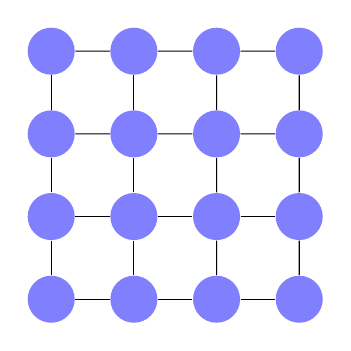
\begin{tikzpicture}[scale=0.7, darkstyle/.style={circle,fill=blue!50,minimum size=17}]
% nodes
  \foreach \x in {0,...,3}
    \foreach \y in {0,...,3} 
       {\pgfmathtruncatemacro{\label}{\x - 5 *  \y +21}
       \node [darkstyle]  (\x\y) at (1.5*\x,1.5*\y) {};} 

% connections
  \foreach \x in {0,...,3}
    \foreach \y [count=\yi] in {0,...,2}  
      \draw (\x\y)--(\x\yi) (\y\x)--(\yi\x) ;

\end{tikzpicture}

\end{center}
  \caption[1]{$4 \times 4$ grid toy model used for an exact inference.}
    \label{fig:grid}
\end{figure}

Initially, the external field was set to $0$ and I considered the case when all couplings have the same value ranging from $-1$ to $1$. As it was expected, the naive mean field approach becomes an upper bound for the variational free energy. However, even in the case of this small model the TAP approximation for different values of couplings is either upper or lower bound. We can see that the approximation is closest to the ground truth when the couplings are close to zero. This is consistent with the fact that the approximation was performed around point where the temperature $T$ is infinite which means that spins are independent -- small values of couplings imitate this state.

Another computational inference problem that can be evaluate thanks to the TAP method is computing a mode of the marginal density for a given spin -- in this case we can estimate average value of the spin under the Boltzmann distribution. The right plot in the Figure \ref{fig:gridModel} shows the mean squared error (MSE) between the real and estimated magnetizations for all spins. In this case, the TAP approach provides much better estimates than the naive method -- we can see that adding a second term to the approximation allows to properly model the connections between the spins in the system. 

\begin{figure}[!htb]
\minipage{0.50\linewidth}%
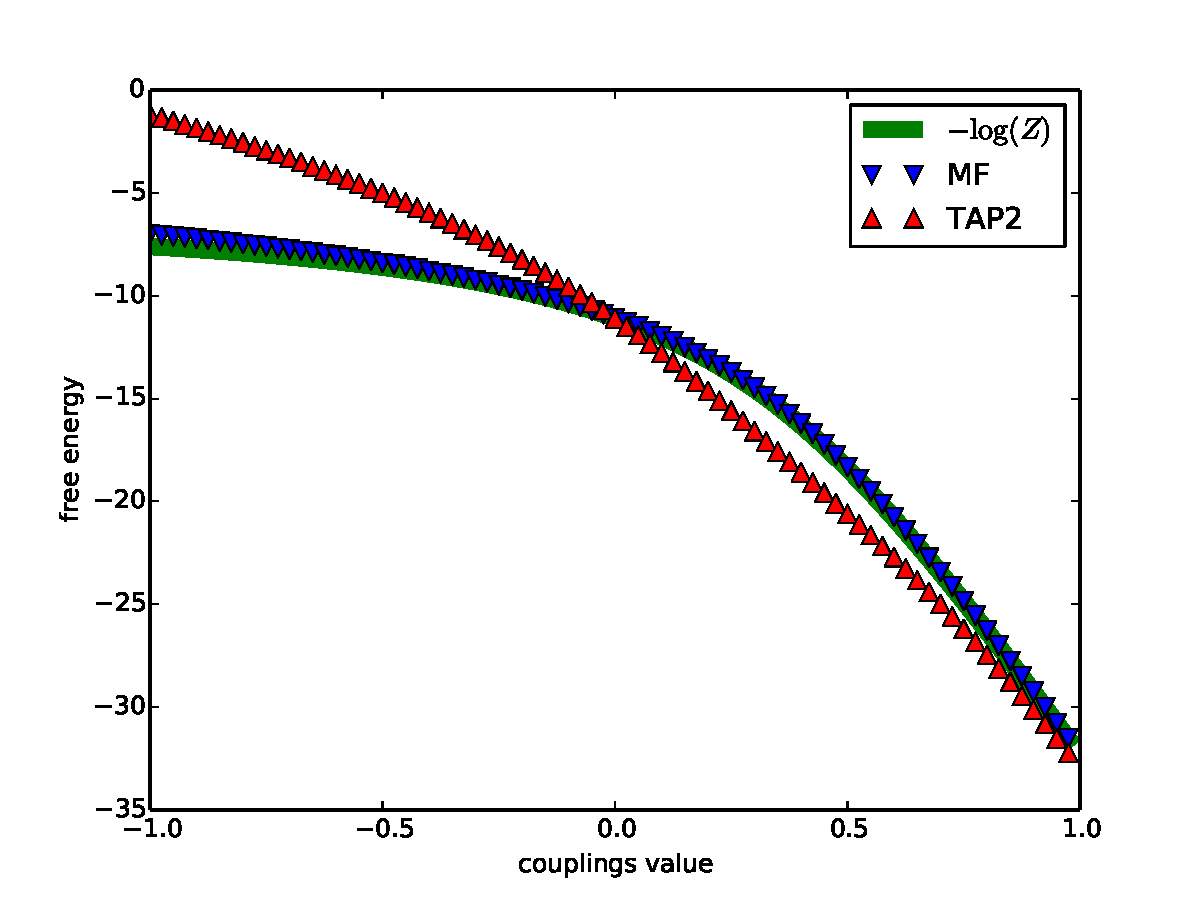
\includegraphics[width=\linewidth]{../../../Code/DRBM/toy/sameCouplingsZ}
\endminipage 
\minipage{0.50\linewidth}  
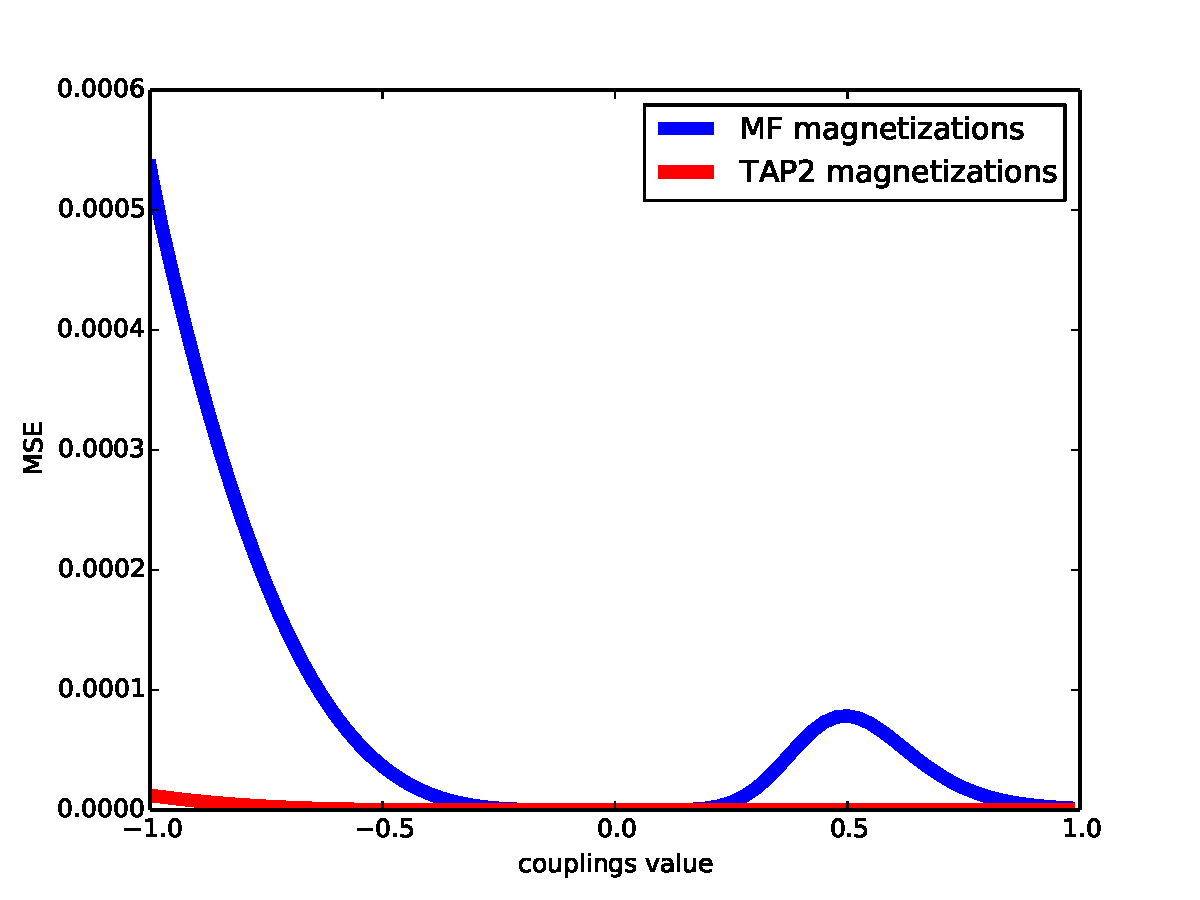
\includegraphics[width=\linewidth]{../../../Code/DRBM/toy/sameCouplingsMAG}
\endminipage\hfill
  \caption[Grid toy model -- the couplings strength]{Comparison of two  variational approaches -- free energy estimates (left) with the true free energy (green line) and MSE between real and estimated magnetisations (right) as a function of the couplings strength ranging from $-1$ to $1$.}
  \label{fig:gridModel}
\end{figure}

In the next experiment, all couplings were initialised to random values around "mean" strength which varies from $0$ to $1$ and then randomly assigned with positive or negative sign. The results are similar to the one observed previously (Figure \ref{fig:gridModelCoup}). The naive approach gives consistently better approximation for the $-\ln Z$ while the TAP method performs better in the case of estimating an average value of spin. 

\begin{figure}[!htb]
\minipage{0.50\linewidth}%
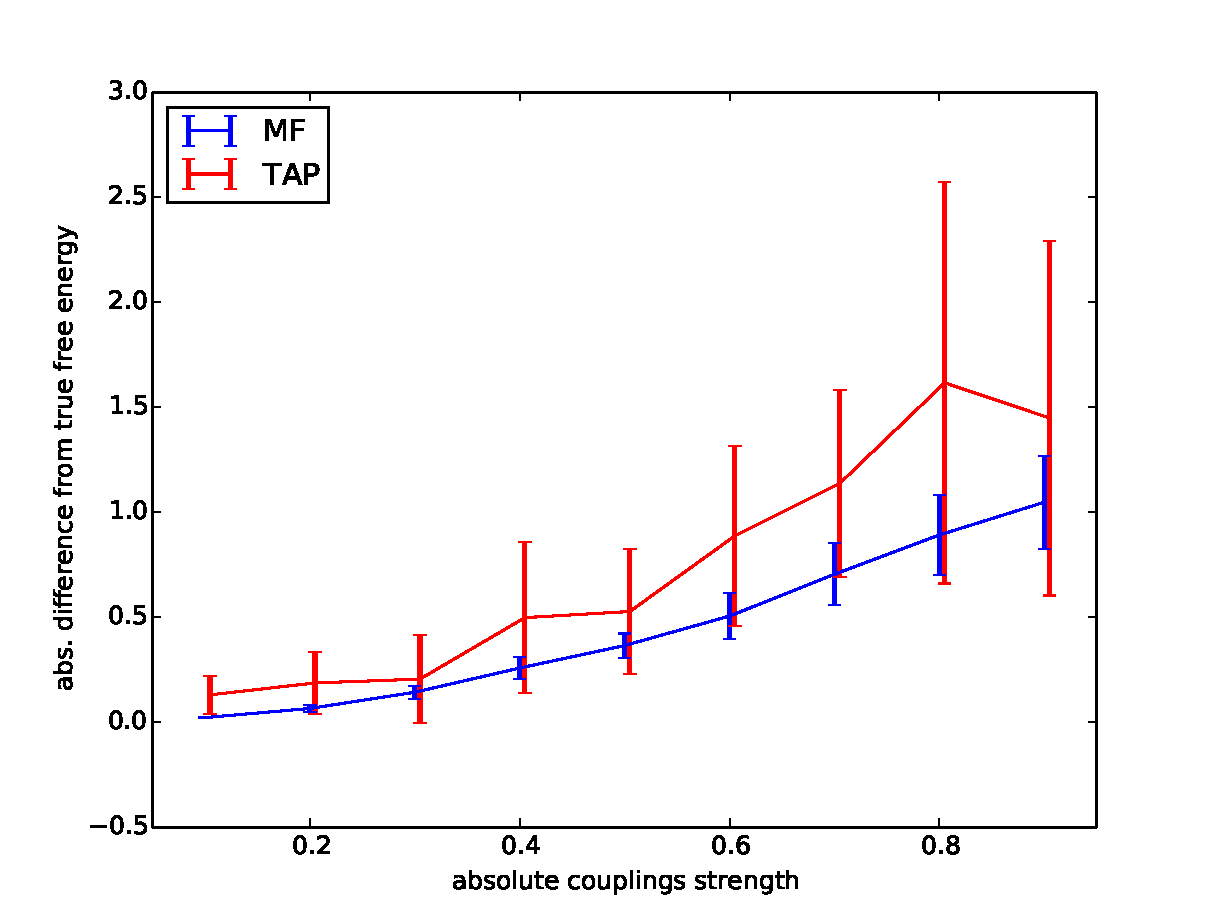
\includegraphics[width=\linewidth]{../../../Code/DRBM/toy/randomWeightsZ}
\endminipage 
\minipage{0.50\linewidth}  
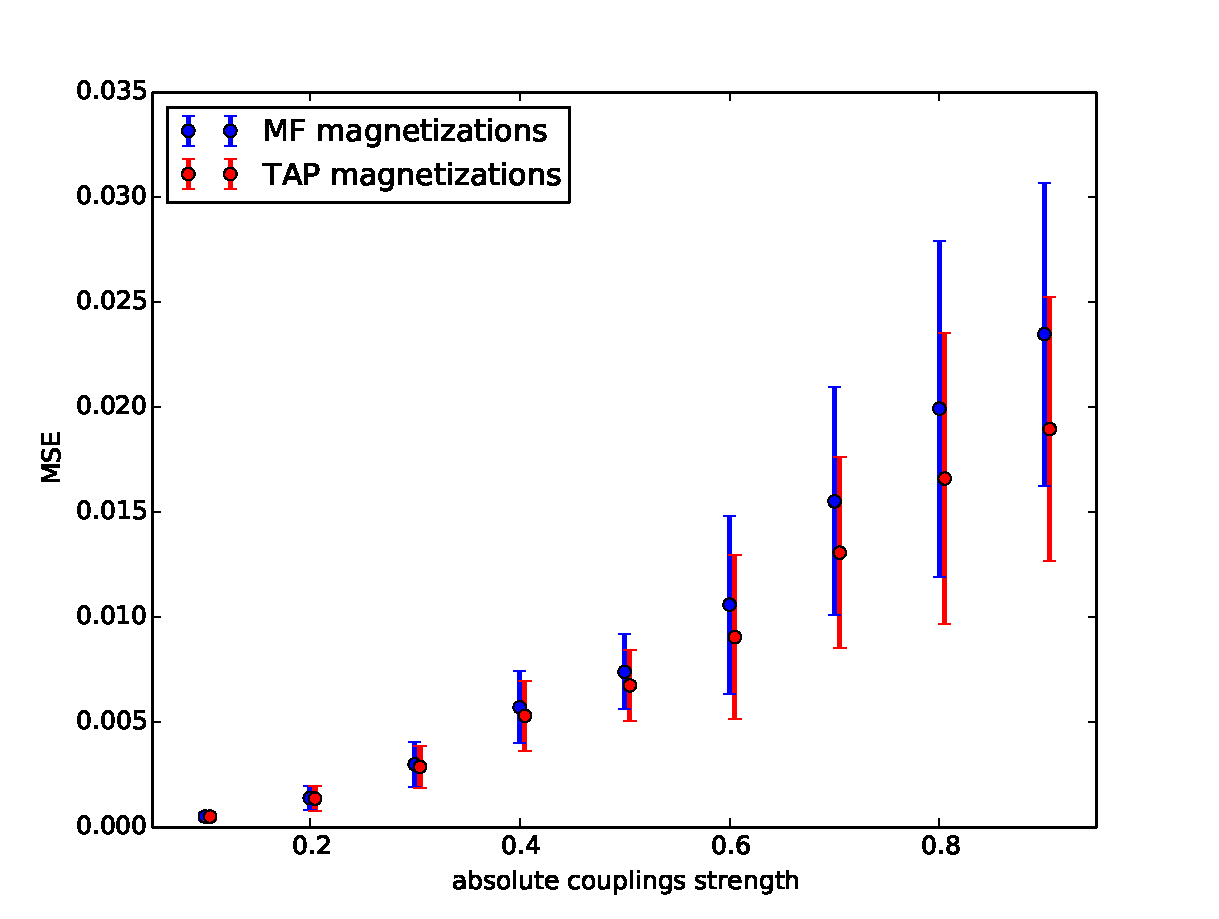
\includegraphics[width=\linewidth]{../../../Code/DRBM/toy/randomWeightsMAG}
\endminipage\hfill
  \caption[1]{Absolute difference between true free energy and the one computed by the naive and the extended mean field approach (left) and MSE between real and estimated magnetisations (right) as a function of the absolute value of couplings strength.}
  \label{fig:gridModelCoup}
\end{figure}

The addition of external fields didn't change substantially the performance of methods  and the results are not included here.

\subsection{RBM toy model}
Due to the different structure of connections between states, the RBM toy model is less trivial to approximate. This should lead to considerably different results in the performance comparing to the toy mode  and it will be an another motivation to use the extended mean field approach on the real data set.

Unlike in the previous case, there is no strong heuristics how the updates of self-consistency relations should be performed. The literature suggests that in the case of the naive approach it is necessary to run self-consistency equations sequentially \cite{welling2002new}. To assess the impact on the final estimates, all three different schedules of updates will be considered here. Following the analysis from the previous section, initially all couplings were set to the same value ranging from $-1$ to $1$  (Figure 5).
\begin{figure}[!htb]
\minipage{0.50\linewidth}%
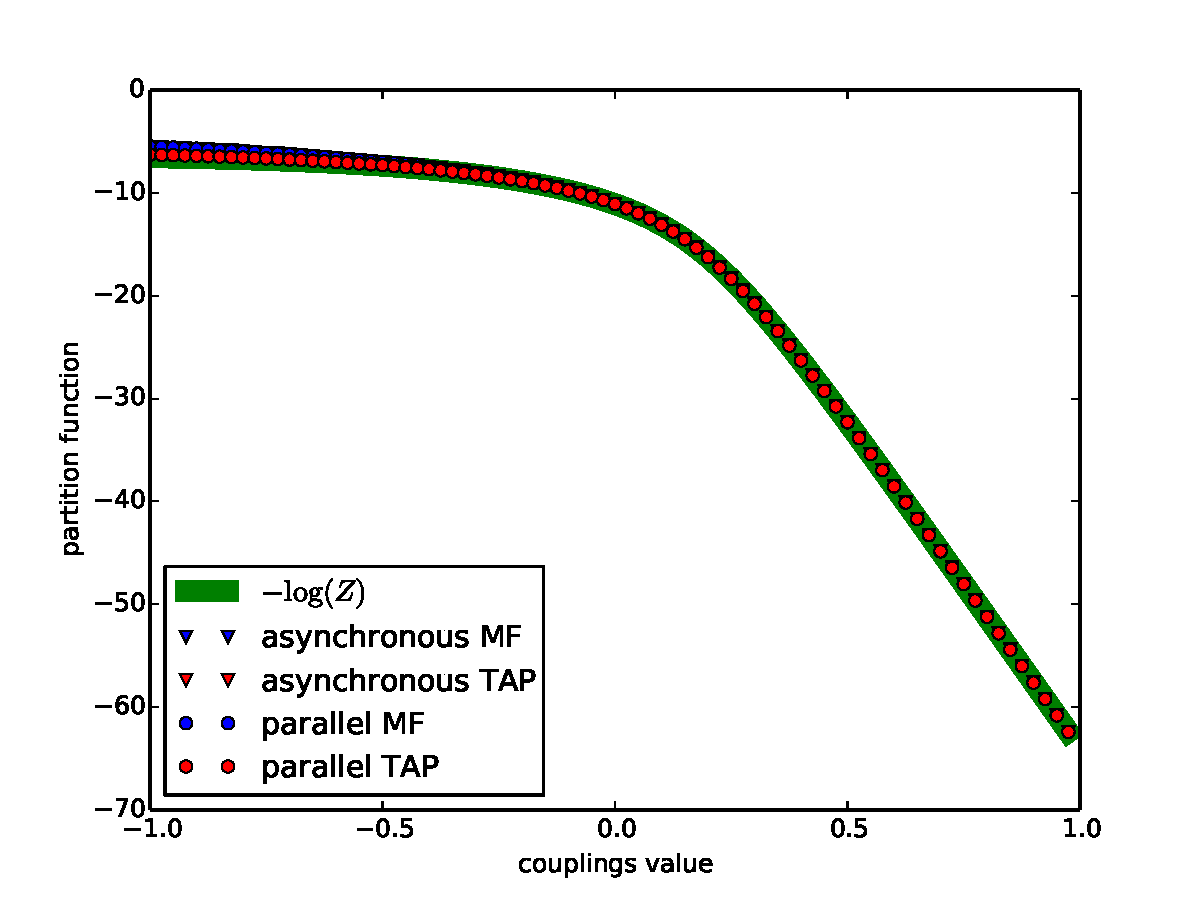
\includegraphics[width=\linewidth]{../../../Code/DRBM/toy/sameCouplingsRBMZ}
\endminipage 
\minipage{0.50\linewidth}  
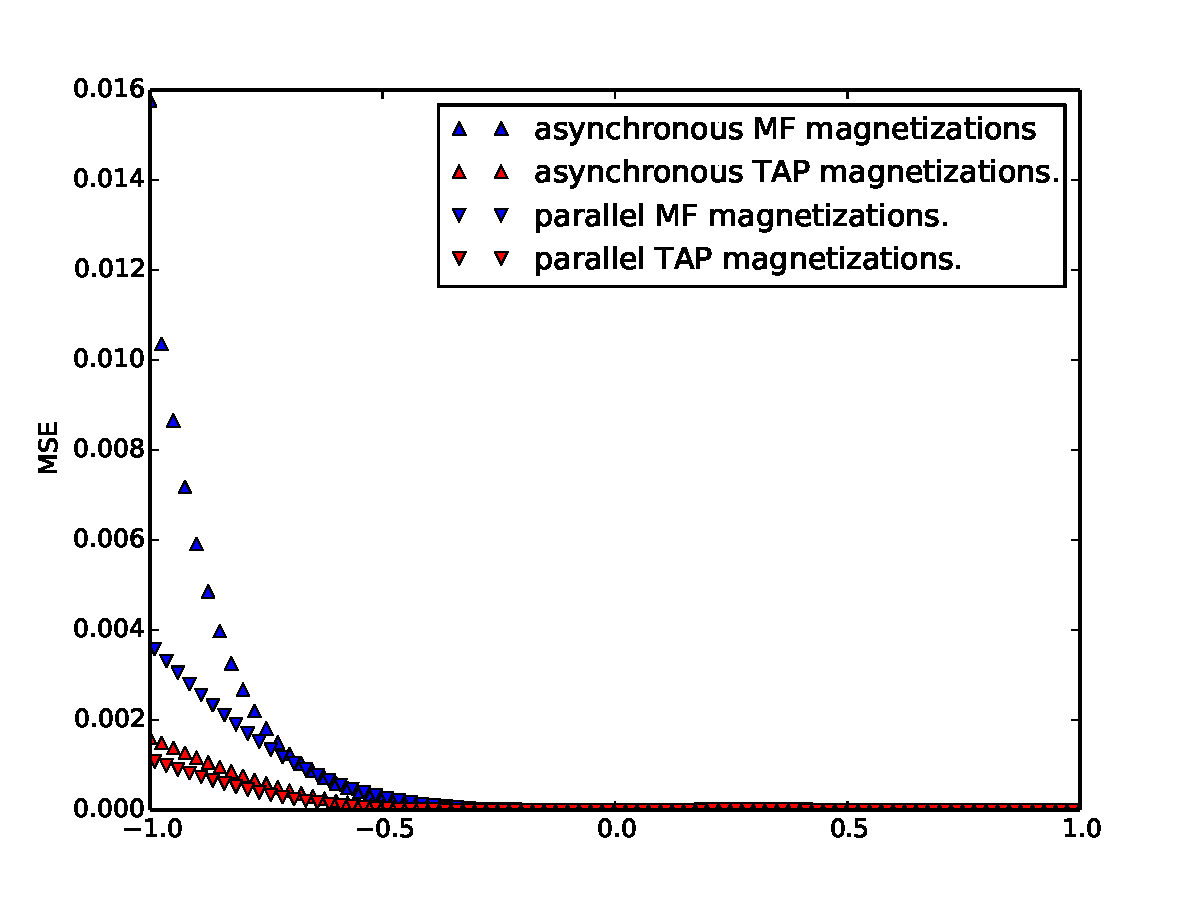
\includegraphics[width=\linewidth]{../../../Code/DRBM/toy/sameCouplingsRBMMAG}
\endminipage\hfill
\label{fig:rbmSame}
  \caption[1]{Comparison of two  variational approaches -- free energy estimates (left)with the true free energy (green line) and MSE between real and estimated magnetisations (right) as a function of the couplings strength ranging from $-1$ to $1$.}
\end{figure}

Unlike the case of the grid model, the estimation of the free energy is almost exact in the case of the TAP method while the naive mean field method again provides a slightly biased upper bound. As it was the case on the grid model, the magnetizations estimated using extended approximation are very precise while MF magnetizations shows discrepancies from true values when connections become stronger in the model. No significant differences were observed between different schedules of updates and thus results for sequential updates weren't included here.

When couplings were random with randomly assigned negative or positive signs, TAP approximation again yields consistently much better estimates that most of the time are exact at the same time having much smaller variance (Figure \ref{fig:rbmRandom}). Again, differences between schedules of updates were negligible and thus the results for sequential updates weren't included as they were almost identical to the ones obtained with asynchronous iterations.
\begin{figure}[!htb]
\minipage{0.50\linewidth}%
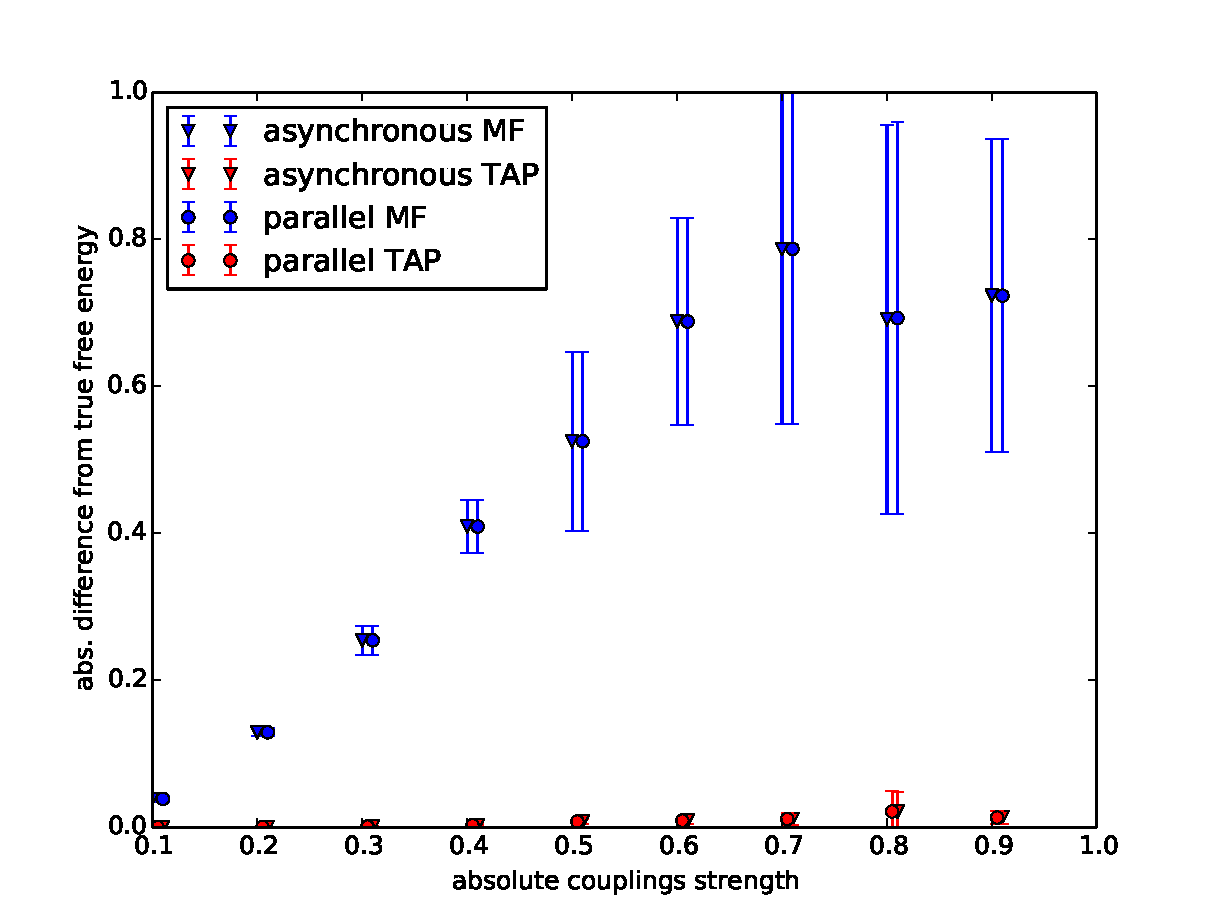
\includegraphics[width=\linewidth]{../../../Code/DRBM/toy/randomWeightsRBMZ}
\endminipage 
\minipage{0.50\linewidth}  
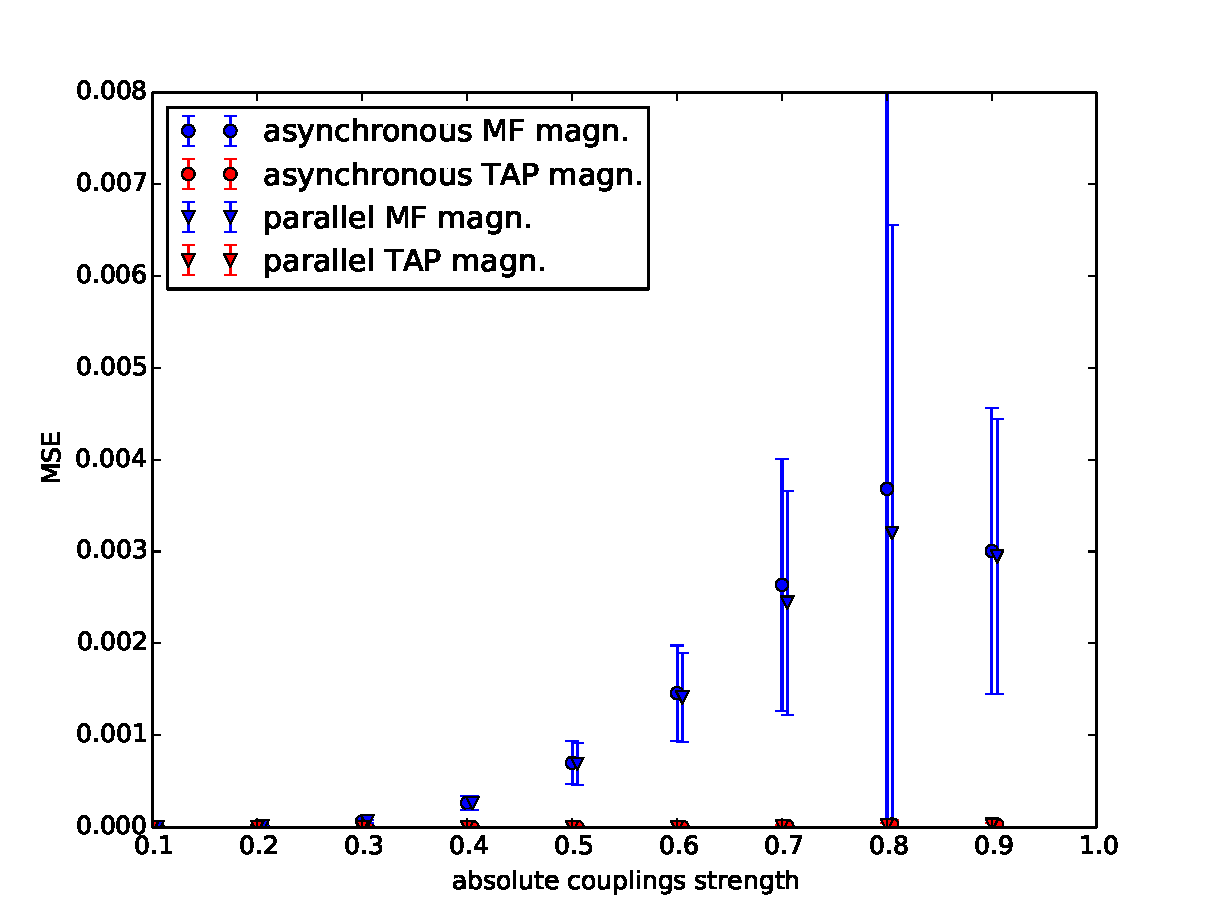
\includegraphics[width=\linewidth]{../../../Code/DRBM/toy/randomWeightsRBMMAG}
\endminipage\hfill
  \caption[1]{Absolute difference between the true free energy and the one computed by the naive and the extended mean field approach (left) and MSE between real and estimated magnetisations (right) as a function of the absolute value of couplings strength.}
  \label{fig:rbmRandom}
\end{figure}

The randomness associated with choosing the sign of connections might have averaged the overall statistics of the model, which in turn might affect the effectiveness of different schedules of updates. Thus, to assess how robust the analysed extended method is with different schedules, the couplings were chosen again randomly around given mean values but this time the sign of the weight was chosen sequentially (Figure \ref{fig:signs}).
\begin{figure}[!htb]
\minipage{0.50\linewidth}%
 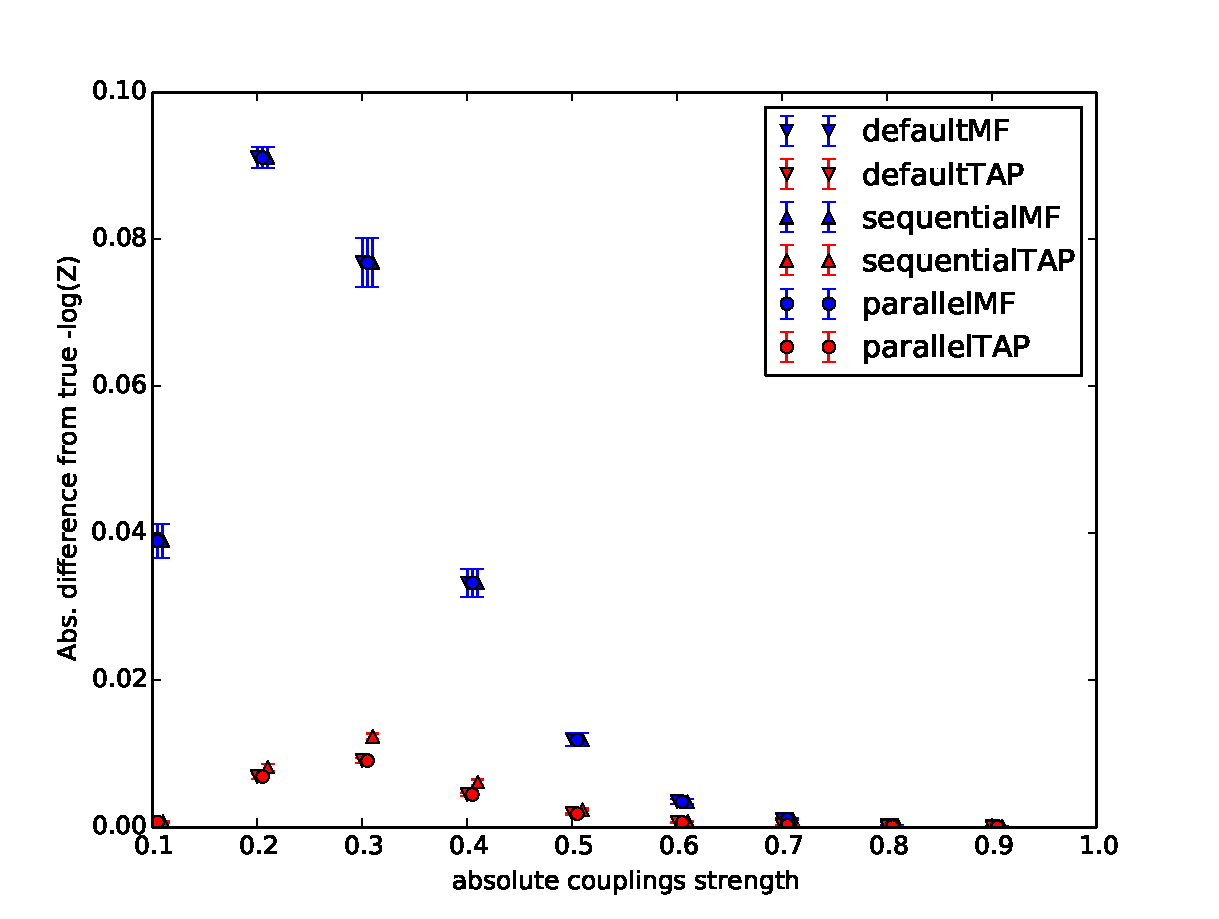
\includegraphics[width=\linewidth]{../../../Code/DRBM/toy/randomWeightsSignsRBMZ}
\endminipage 
\minipage{0.50\linewidth}  
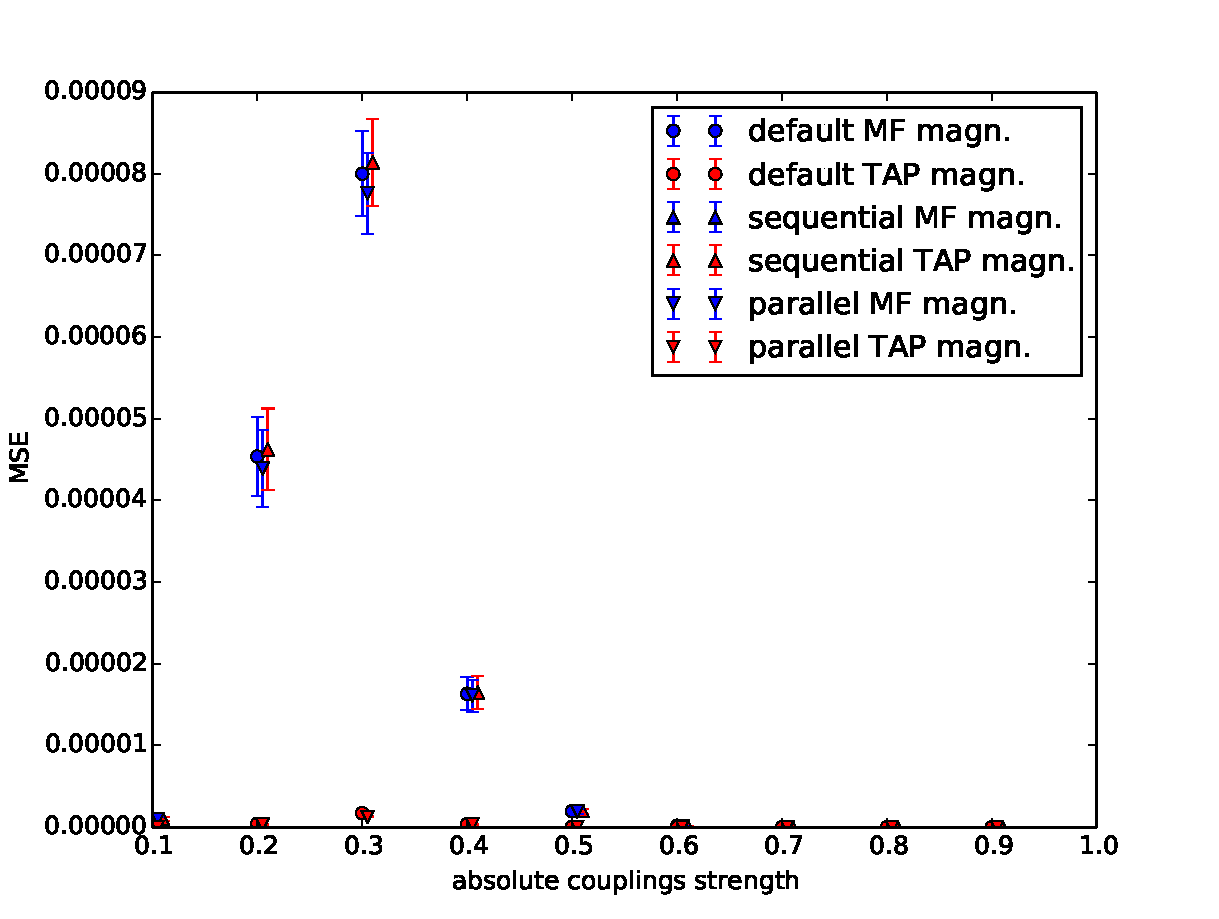
\includegraphics[width=\linewidth]{../../../Code/DRBM/toy/randomWeightsSignsRBMMAG}
\endminipage\hfill
  \caption[1]{Absolute difference between the true free energy and the one computed by the naive and the extended mean field approach (left) and MSE between real and estimated magnetisations (right) as a function of the absolute value of couplings strength with sequentially opposite signs.}
  \label{fig:signs}
\end{figure}

This time, TAP estimates are not exact for couplings with an absolute strength around values $0.2$ or $0.3$. Moreover, the sequential updates yield very poor estimates for the magnetizations -- the MSE is almost the same as with the naive approach. The addition of external fields this time extensify the differences in performance between updates (Figure \ref{fig:bias}). The MSE between true and estimated magnetizations is higher for the TAP model with sequential updates than for the corresponding naive model.

\begin{figure}[!htb]
\minipage{0.50\linewidth}%
 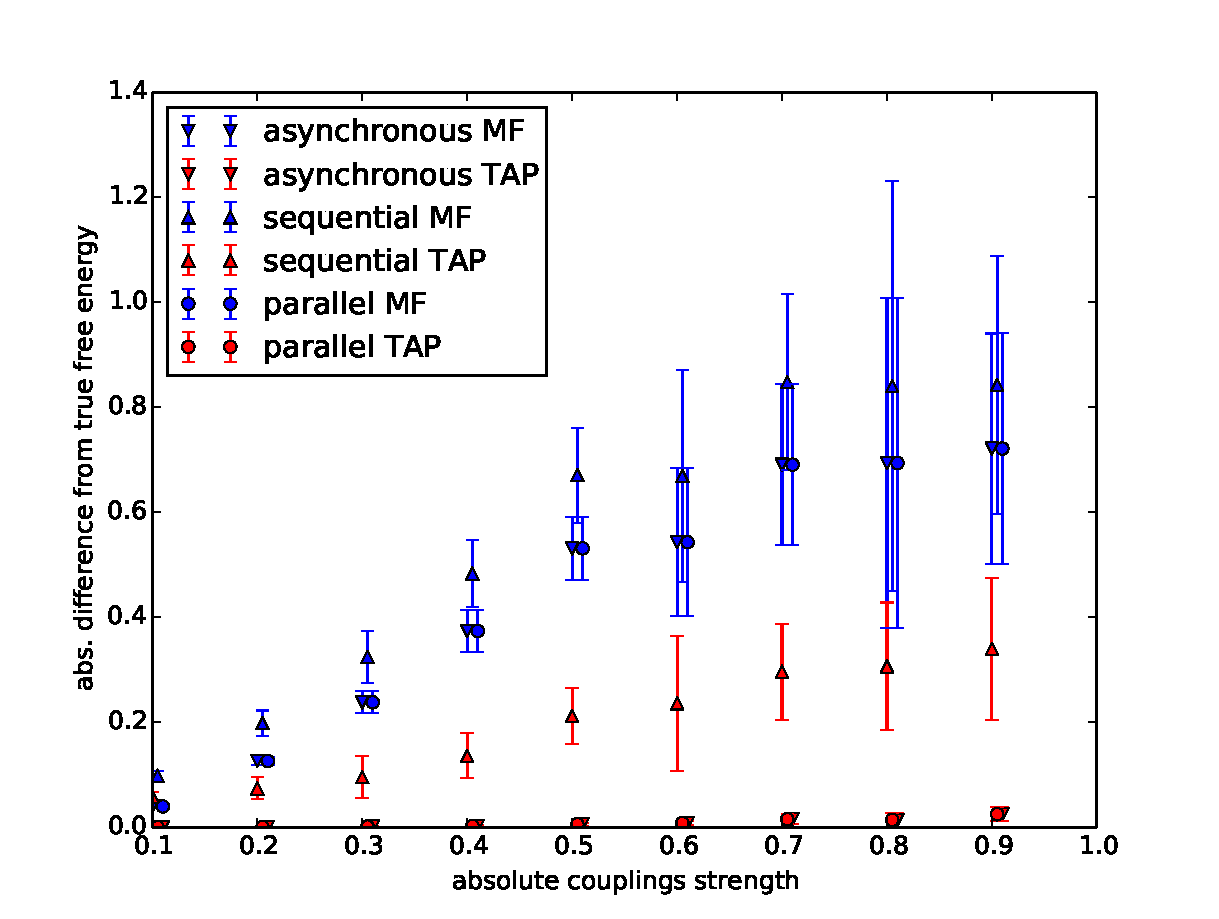
\includegraphics[width=\linewidth]{../../../Code/DRBM/toy/BrandomWeightsRBMZ}
\endminipage 
\minipage{0.50\linewidth}  
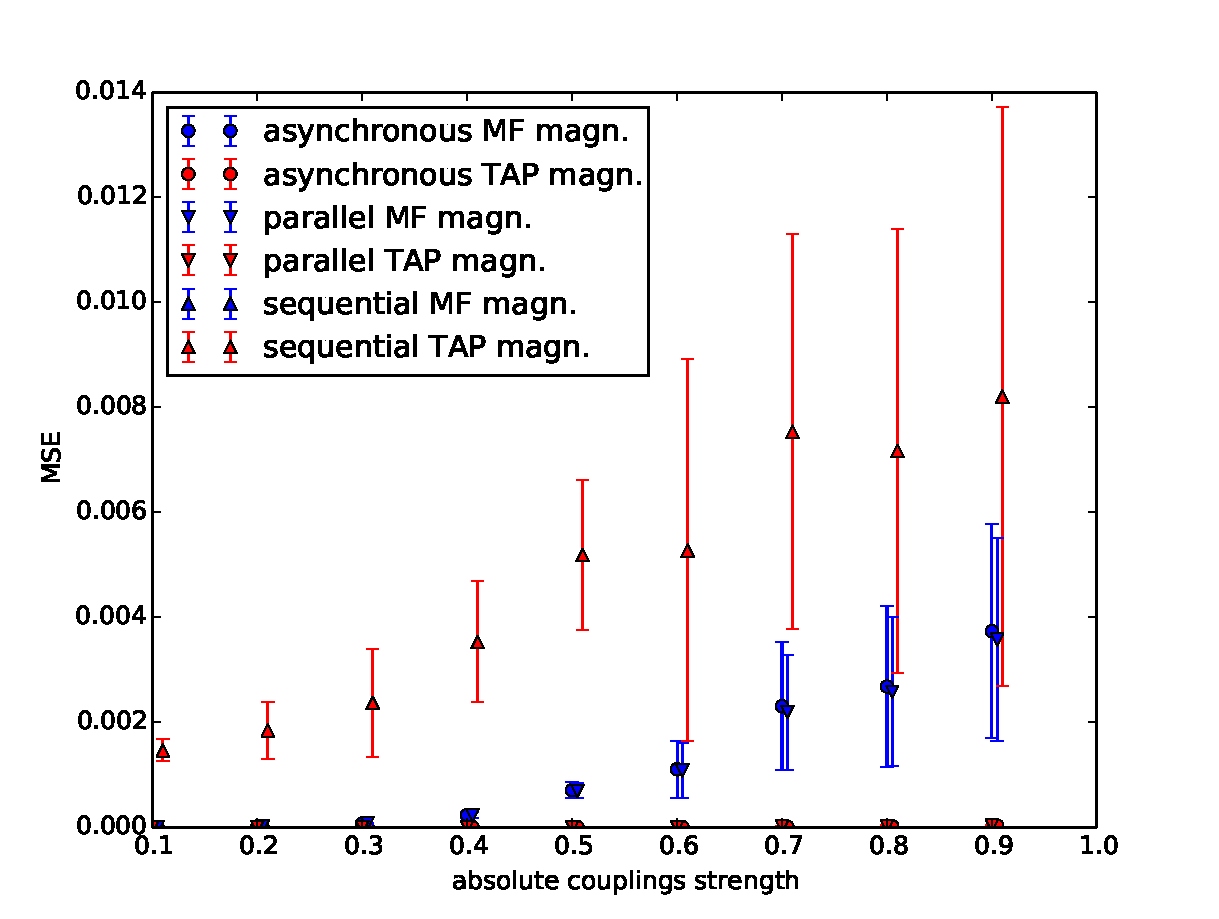
\includegraphics[width=\linewidth]{../../../Code/DRBM/toy/BrandomWeightsRBMMAG}
\endminipage\hfill
  \caption[1]{Absolute difference between true free energy and the one computed by naive and extended mean field approach (left) an MSE between real and estimated magnetisations (right) as a function of the absolute value of couplings strength with sequential changes of signs.}
  \label{fig:bias}
\end{figure}

Taking into consideration all results we can infer that the extended approximation yields robust results even though the expansion is performed at $\beta = 1$ and the couplings between the spins might have strong connections. Moreover, the real benefits of modelling the relationship between the spins can be observed when the MRF has the RBM structure. In this case the estimates of the free energy and the magnetizations were almost exact for the EMF-based model. However, contrary to the heuristics parallel updates perform just as well as the asynchronous ones while the sequential updates might drastically worsen the quality of estimates for the EMF-based models.

